\documentclass{article}

\usepackage{arxiv}

\usepackage[utf8]{inputenc} % allow utf-8 input
\usepackage[T1]{fontenc}    % use 8-bit T1 fonts
\usepackage[hidelinks]{hyperref}       % hyperlinks
\usepackage{url}            % simple URL typesetting
\usepackage{booktabs}       % professional-quality tables
\usepackage{amsmath,amssymb,amsthm}
\usepackage{amsfonts}       % blackboard math symbols
\usepackage{nicefrac}       % compact symbols for 1/2, etc.
\usepackage{microtype}      % microtypography
\usepackage{mathrsfs}
\usepackage{onimage}
\usepackage{graphicx}
\usepackage{doi}
\usepackage{acronym}
\usepackage{listings}
\usepackage{tikz}

\usetikzlibrary{trees}

\title{
    A mechanical Model of Rod-Shaped Bacteria
}

%\date{September 9, 1985}	% Here you can change the date presented in the paper title
%\date{} 					% Or removing it

\author{
    \href{https://orcid.org/0009-0001-0613-7978}{
        
\includegraphics[scale=0.06]{orcid.pdf}
        \hspace{1mm}Jonas Pleyer
    }
    \thanks{
        \href{https://jonas.pleyer.org}{jonas.pleyer.org},
        \href{https://cellular-raza.com}{cellular-raza.com}
    }\\
	Freiburg Center for Data-Analysis and Modeling\\
	University of Freiburg\\
	\texttt{jonas.pleyer@fdm.uni-freiburg.de} \\
	%% examples of more authors
	\And
	\href{https://orcid.org/0000-0002-6371-4495}{
        
\includegraphics[scale=0.06]{orcid.pdf}
        \hspace{1mm}Christian Fleck
    }\\
	Freiburg Center for Data-Analysis and Modeling\\
	University of Freiburg
}

% Uncomment to remove the date
%\date{}

% Uncomment to override  the `A preprint' in the header
\renewcommand{\headeright}{Preprint}
%\renewcommand{\undertitle}{Technical Report}
\renewcommand{\shorttitle}{A mechanical Model of Rod-Shaped Bacteria}

\usepackage{enumitem}
\setlist{nolistsep}

%%% Add PDF metadata to help others organize their library
%%% Once the PDF is generated, you can check the metadata with
%%% $ pdfinfo template.pdf
\hypersetup{
pdftitle={% TODO
},
pdfsubject={q-bio.NC, q-bio.QM},
pdfauthor={Jonas Pleyer, Christian Fleck},
pdfkeywords={},
}

% Change numbering of equations
% \numberwithin{equation}{section}

% MAKE TITLES IN THEOREMS BOLD
\makeatletter
\def\th@plain{%
  \thm@notefont{}% same as heading font
  \itshape % body font
}
\def\th@definition{%
  \thm@notefont{}% same as heading font
  \normalfont % body font
}
\makeatother

\begin{document}
\maketitle

%###################################################################################################
\begin{abstract}
    This paper develops the formal notions of cellular \dots
\end{abstract}

% keywords can be removed
% \keywords{}

%###################################################################################################
\section{Introduction}
\label{section:introduction}

%###################################################################################################
\section{A mechanical Model of Rod-Shaped Bacteria}
\label{section:mechanical-model-rod-shaped-bacteria}

Bacteria exist in many physical shapes such as spheroidal, rod-shaped or spiral
\cite{Zapun2008,Young2006}.

To model the spatial mechanics of elongated bacteria \cite{Billaudeau2017}, we represent them as a
collection of auxiliary vertices $\{\vec{v}_i\}$ which are connected by springs in
ascending order.
Furthermore, we assume that the cells are flexible described by their rigidity.
A force $\vec{F}$ interacting between cellular agents determines the radius (thickness) of the
rods and an attractive component can model adhesion between cells.

% --------------------------------------------------------------------------------------------------
\subsection{Mechanics}

%TODO use these citations
\cite{Chatterjee1988},\cite{Ursell2014}

In principle we can assign individual lengths $\{l_i\}$ and strengths $\{\gamma\}_i$ to each spring.
The internal force acting on vertex $\vec{v}_i$ can be divided into 2 contributions coming
from the 2 springs pulling on it.
In the case when $i=0,N_\text{vertices}$, this is reduced to only one internal component.
We denote with $\vec{c}_{i}$ the connection between two vertices

\begin{equation}
    \vec{c}_i = \vec{v}_{i}-\vec{v}_{i-1}
\end{equation}

and can write down the resulting force

\begin{align}
    \vec{F}_{i,\text{springs}} =
        &-\gamma_i\left(1 - \frac{l_i}{\left|\vec{c}_i\right|}\right)\vec{c}_i\\
        &+ \gamma_{i+1}\left(1 - \frac{l_{i+1}}{\left|\vec{c}_{i+1}\right|}\right)\vec{c}_{i+1}
    \label{force-springs}
\end{align}

In addition to springs between individual vertices $\vec{v}_i$, we assume that each angle at
a vertex between two other is subject to a curvature force.
Assuming that $\alpha_i$ is the angle between the connections and
$\vec{d}_i=\vec{c}_i/|\vec{c}_i|$ is the normalized connection,
we can write down the forces acting on vertices $\vec{v}_i,\vec{v}_{i-1},\vec{v}_{i+1}$

\begin{align}
    \vec{F}_{i,\text{curvature}} &= \eta_i\tan\left(\pi-\alpha_i\right)
        \frac{\vec{d}_i - \vec{d}_{i+1}}{|\vec{d}_i-\vec{d}_{i+1}|}\\
    \vec{F}_{i-1,\text{curvature}} &= -\frac{1}{2}\vec{F}_{i,\text{curvature}}\\
    \vec{F}_{i+1,\text{curvature}} &= -\frac{1}{2}\vec{F}_{i,\text{curvature}}
    \label{force-curvature}
\end{align}

where $\eta_i$ is the curvature at vertex $\vec{v}_i$.
We can see that the curvature force does not move the overall center of the cell in space.

\begin{figure}
    \centering
    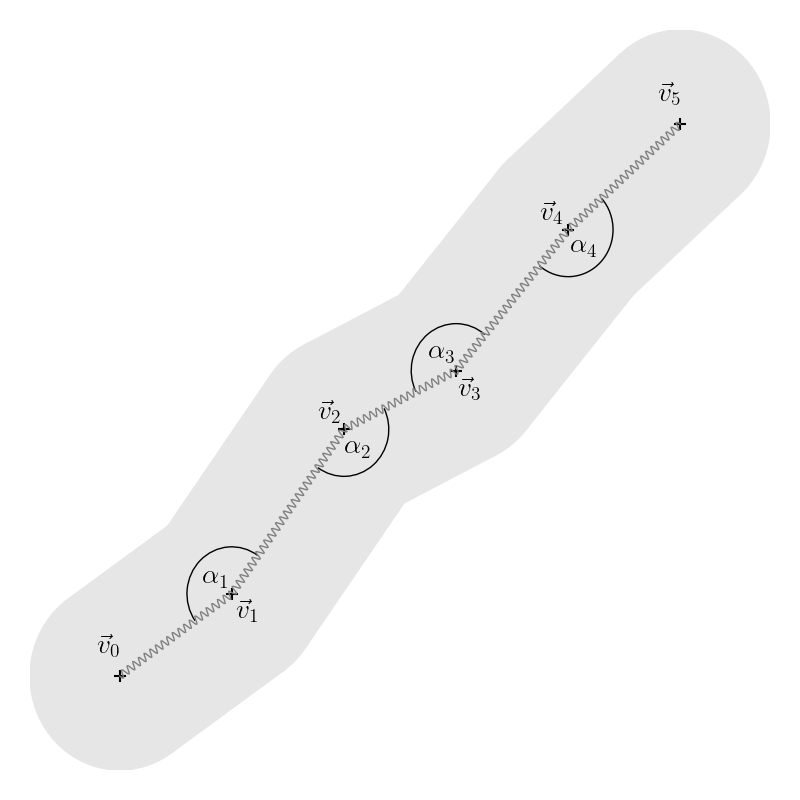
\includegraphics[width=0.5\textwidth]
        {../docs/source/_static/mechanics.png}
    \caption{Example of a polygonal representation of a rod-shaped bacterium.}
    \label{fig:mechanics-bacterium}
\end{figure}

The total force is the sum of external and interal forces.

\begin{equation}
    \vec{F}_{i,\text{total}} = \vec{F}_{i,\text{springs}}+ \vec{F}_{i,\text{curvature}} + \vec{F}_{i,\text{external}}
   \label{force-total}
\end{equation}

and are integrated via

\begin{align}
    \partial_t^2 \vec{x} &= \partial\vec{x} + D\vec{\xi}\\
    \partial_t\vec{x} &= \vec{F}_\text{total}
    \label{equations-of-motion}
\end{align}

where $D$ is the diffusion constant and  $\vec{\xi}$ is the wiener process (compare with
brownian motion such as given by the
% Brownian3D <https://cellular-raza.com/docs/cellular_raza_building_blocks/struct.Brownian3D.html>_
% struct of cellular-raza <https://cellular-raza.com>.

% --------------------------------------------------------------------------------------------------
\subsection{Interaction}

When calculating forces acting between the cells, we can use a simplified model to circumvent the
numerically expensive integration over the complete length of the rod.
Given a vertex $\vec{v}_i$ on one cell, we calculate the closest point $\vec{p}$ on the polygonal
line given by the vertices $\{\vec{w}_j\}$ of the interacting cell.
Furthermore we determine the value $q\in[0,1]$ such that

\begin{equation}
    \vec{p} = (1-q)\vec{w}_j + q\vec{w}_{j+1}
   \label{connection}
\end{equation}

for some specific $j$.
The force is then calculated between the points $\vec{v}_i$ and $\vec{p}_i$ and acts on
the vertex $\vec{w}_i,\vec{w}_{i+1}$ with relative strength $(1-q)$ and $q$.

\begin{equation}
    \vec{F}_{i,\text{External}} = \vec{F}(\vec{v}_i,\vec{p})
    \label{force-external}
\end{equation}

% .. _ TODO MORSEPOTENTIAL

% .. _ TODO insert table with all parameters

% --------------------------------------------------------------------------------------------------
\subsection{Cycle}

To simulate proliferation, we introduce a growth term for the spring lengths $l_i$

\begin{equation}
    \partial_t l_i = \mu
    \label{growth-ode}
\end{equation}

which will increase the length of the cell indefenitely unless we introduce a
% `division event <https://cellular-raza.com/internals/concepts/cell/cycle>`_.
We define a threshold (in our case double of the original length) for the total length of the
cell at which it divides.
To construct a new cell, we cannot simply copy the existing one twice, but we also need to adjust
internal parameters in the process.
The following actions need to be taken for the old and new agent.

% .. _ TODO

1. Assign a new growth rate (pick randomly from uniform distribution in $[0.8\mu_0,1.2\mu_0]$
   where $\mu_0$ is some fixed value)
2. Assign new positions
    1. Calculate new spring lengths
        $\tilde{l}_i = l_i\left(\frac{1}{2} - \frac{r}{\sum\limits_i l_i}\right)$
    2. Calculate middle of old cell
        $\vec{m} = \frac{1}{N_\text{vertices}}\sum\limits_i\vec{v}_i$
    3. Calculate positions of new vertices $\vec{w}_i$

\begin{align}
    q_i &= \frac{i}{N_\text{vertices}}\\
    \vec{w}_{i,\text{new},\pm} &= (1-q_i)\vec{m} + q_i(\vec{v}_{\pm\text{start}} - \vec{m})
\end{align}

%###################################################################################################
\section{Generating Masks and Images}
\label{section:generating-masks-and-images}

\begin{figure}
    \centering
    \begin{tikzonimage}[width=0.3\textwidth]
        {../docs/source/_static/09395645494836445480/raw_pv/000000400.png}
        \node at (0.025, 0.975)[anchor=north west, rectangle, draw, white, minimum width=15pt, minimum height=15pt]{\textbf{a}};
    \end{tikzonimage}
    \begin{tikzonimage}[width=0.3\textwidth]
        {../docs/source/_static/09395645494836445480/images/000000400.png}
        \node at (0.025, 0.975)[anchor=north west, rectangle, draw, white, minimum width=15pt, minimum height=15pt]{\textbf{b}};
    \end{tikzonimage}
    \begin{tikzonimage}[width=0.3\textwidth]
        {../docs/source/_static/09395645494836445480/masks/000000400.png}
        \node at (0.025, 0.975)[anchor=north west, rectangle, draw, white, minimum width=15pt, minimum height=15pt]{\textbf{c}};
    \end{tikzonimage}
    \caption{Snapshots at \dots}
    \label{fig:progression-image-generation}
\end{figure}

%###################################################################################################
\section{Extract Positions from Masks}
\label{section:fitting-and-comparing-masks}

\begin{figure}
    \centering
    \begin{tikzonimage}[width=0.32\textwidth]
        {../docs/source/_static/fitting-methods/algorithm/image001042.png}
        \node at (0.025, 0.975)[anchor=north west, rectangle, draw, white, minimum width=15pt, minimum height=15pt]{\textbf{a}};
    \end{tikzonimage}
    \begin{tikzonimage}[width=0.32\textwidth]
        {../docs/source/_static/fitting-methods/algorithm/mask-zoom.png}
        \node at (0.025, 0.975)[anchor=north west, rectangle, draw, white, minimum width=15pt, minimum height=15pt]{\textbf{b}};
    \end{tikzonimage}
    \begin{tikzonimage}[width=0.32\textwidth]
        {../docs/source/_static/fitting-methods/algorithm/mask-zoom.png}
        \node at (0.025, 0.975)[anchor=north west, rectangle, draw, white, minimum width=15pt, minimum height=15pt]{\textbf{c}};
    \end{tikzonimage}
    \caption{}
    \label{fig:position-extraction-algorithm}
\end{figure}

\begin{figure}
    \centering
    \begin{tikzonimage}[width=0.32\textwidth]
        {../docs/source/_static/fitting-methods/extract_positions-000400.png}
        \node at (0.025, 0.975)[anchor=north west, rectangle, draw, white, minimum width=15pt, minimum height=15pt]{\textbf{a}};
    \end{tikzonimage}
    \begin{tikzonimage}[width=0.32\textwidth]
        {../docs/source/_static/fitting-methods/extract_positions-000600.png}
        \node at (0.025, 0.975)[anchor=north west, rectangle, draw, white, minimum width=15pt, minimum height=15pt]{\textbf{b}};
    \end{tikzonimage}
    \begin{tikzonimage}[width=0.32\textwidth]
        {../docs/source/_static/fitting-methods/extract_positions-001200.png}
        \node at (0.025, 0.975)[anchor=north west, rectangle, draw, white, minimum width=15pt, minimum height=15pt]{\textbf{c}};
    \end{tikzonimage}
    \caption{Progression of generated masks with estimated and exact positions.}
    \label{fig:position-extraction}
\end{figure}

\begin{figure}
    \centering
    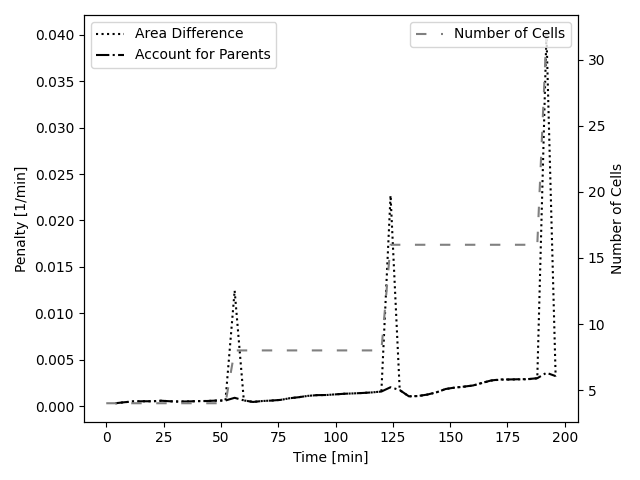
\includegraphics[width=0.5\textwidth]
        {../docs/source/_static/fitting-methods/penalty-time-flow.png}%
    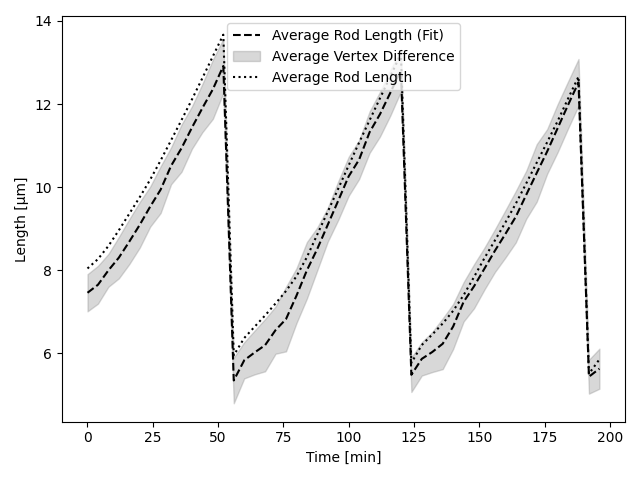
\includegraphics[width=0.5\textwidth]
        {../docs/source/_static/fitting-methods/displacement-calculations.png}
    \caption{Comparison of masks across generations. Compare estimated with exact rod lengths.}
    \label{fig:benchmarking-fitting-algorithm}
\end{figure}

\begin{figure}
    \centering
    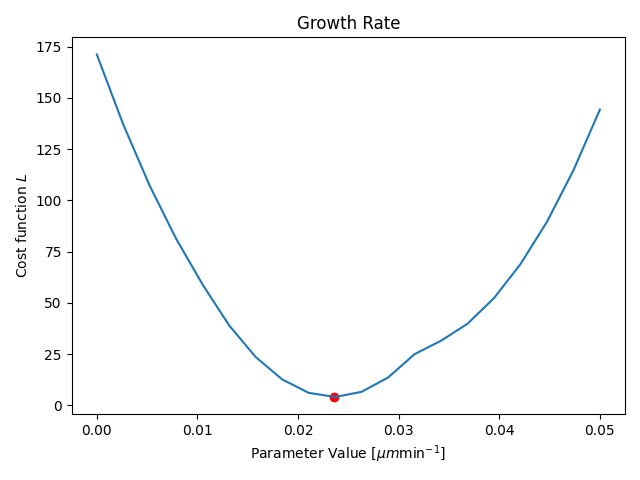
\includegraphics[width=0.32\textwidth]
        {../docs/source/_static/fitting-methods/estimate-parameters1/Growth Rate.png}%
    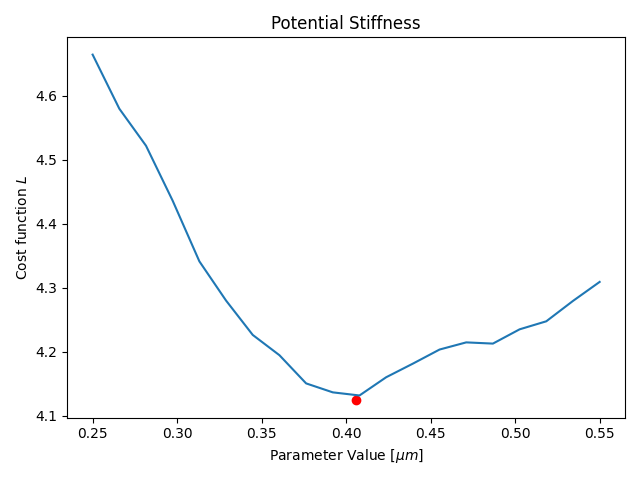
\includegraphics[width=0.32\textwidth]
        {../docs/source/_static/fitting-methods/estimate-parameters1/Potential Stiffness.png}%
    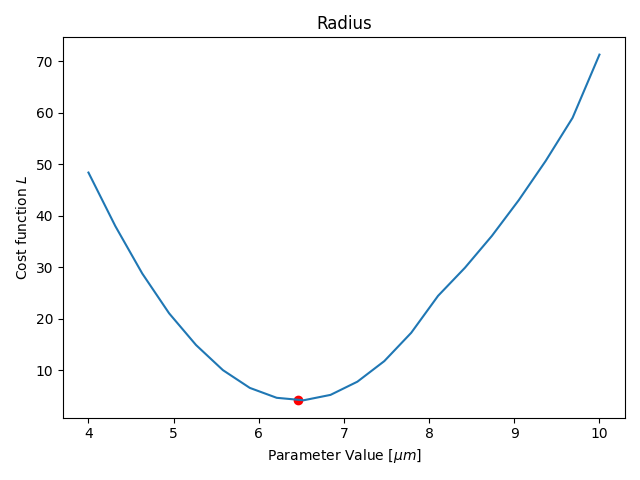
\includegraphics[width=0.32\textwidth]
        {../docs/source/_static/fitting-methods/estimate-parameters1/Radius.png}\\%
    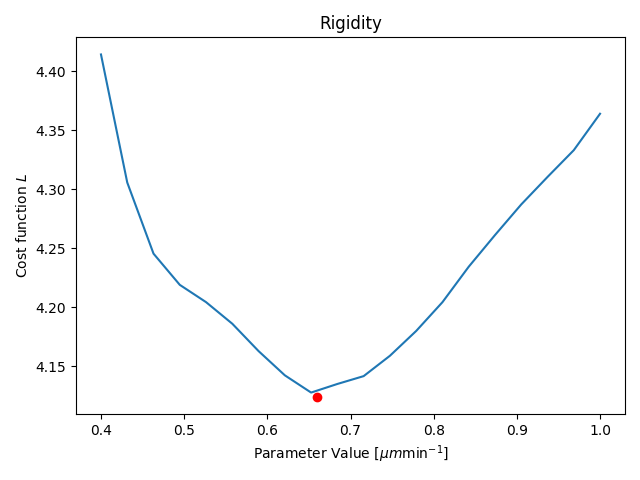
\includegraphics[width=0.32\textwidth]
        {../docs/source/_static/fitting-methods/estimate-parameters1/Rigidity.png}%
    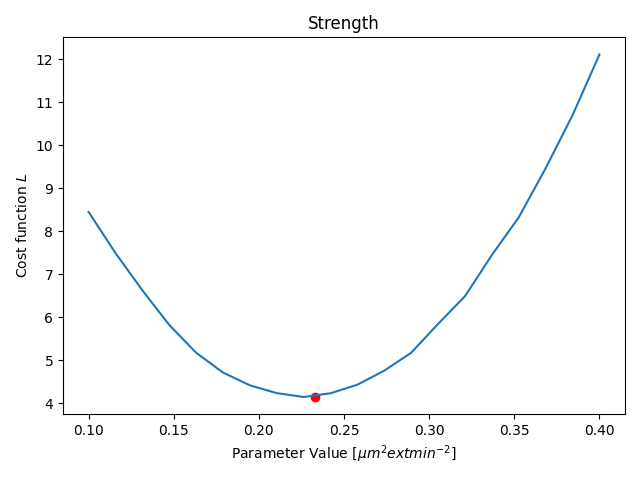
\includegraphics[width=0.32\textwidth]
        {../docs/source/_static/fitting-methods/estimate-parameters1/Strength.png}%
    \caption{Snapshots at \dots}
    \label{fig:parameter-estimates-single-step}
\end{figure}

%###################################################################################################
\section{Estimating Parameters}
\label{section:parameter-estimation}


\bibliographystyle{IEEEtran}
\bibliography{../docs/source/references}

\end{document}
